\chapter{Learning the basics}
In this chapter we'll learn very basics to getting started; so downloading Hazelcast, configuring Hazelcast in a Maven project. And we'll also deal with the different configuration mechanisms of Hazelcast and configuration tricks like wildcard configuration.

\section{Installing Hazelcast}
Hazelcast relies on Java 5, but the examples rely on Java 7. So if you want to compile the examples, make sure Java 7 is installed. If not installed, it can be downloaded from the Oracle site: http://java.com/en/download/index.jsp.

Hazelcast can be downloaded from http://www.hazelcast.com/downloads.jsp and you can choose between 2 versions:
[Talip: Do not mention anthing about Enterprise Edition as we might change our model to be entirely open source]

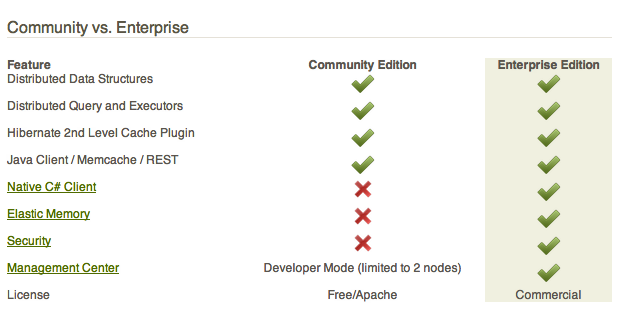
\includegraphics[scale=0.60]{hazelcast-editions.png}

For the purpose of this book we'll use the community edition. If your project relies on Maven, there is no need to install Hazelcast at all, see [link to Hazelcast and Maven]. Otherwise make sure that the Hazelcast jar is added to the classpath. Apart from this jar, there is no need to install Hazelcast.  The lack of an installation process for Hazelcast is something I really like because it saves quite a lot of time, time that can be used to solve real problems instead of environmental ones.

\section{Hazelcast and Maven}
Hazelcast is very easy to include in your Maven 3 project without needing to go through a complex installation process. Hazelcast can be found in the standard Maven repositories, so you do not need to add additional repositories to the pom. To include Hazelcast in your project, just add the following to your pom:
\begin{lstlisting}[language=xml]
<dependencies>	
   <dependency>
      <groupId>com.hazelcast</groupId>
      <artifactId>hazelcast</artifactId>
      <version>3.0</version>
   </dependency>
</dependencies>
\end{lstlisting}
That is it. Make sure that you check the Hazelcast website to make use of the most recent version. After this dependency is added, Maven will automatically downloaded the dependencies needed.

\section{Configuring Hazelcast}
Hazelcast can be configured in different ways:
\begin{enumerate}
\item programmatic configuration
\item XML configuration 
\item Spring configuration
\end{enumerate}
The programmatic configuration is the most essential one, the other mechanisms are build on top of it. In this book we'll use the xml configuration file since that is the shortest. When you are running a Maven project; just add a resources directory under src/main/ and add a file 'hazelcast.xml'. The following shows an empty configuration:
\begin{lstlisting}[language=xml]
<hazelcast 
   xsi:schemaLocation="http://www.hazelcast.com/schema/config                               
      http://www.hazelcast.com/schema/config/hazelcast-config-3.0.xsd"
   xmlns="http://www.hazelcast.com/schema/config"
      xmlns:xsi="http://www.w3.org/2001/XMLSchema-instance">
</hazelcast>
\end{lstlisting}
This example also imports an XML schema (XSD) for validation and if you are using an IDE, you probably get code completion. To reduce the size of the examples in the book, only the elements inside the <hazelcast> tags are provided. In the sources for the book you can find the full xml configuration. Another thing you might run into is the strange formatting of the java code; this is also done to reduce the size. 

In most of our examples we will rely on multicast for member discovery so that the members will join the cluster:
\begin{lstlisting}[language=xml]
<network>
   <join><multicast enabled="true"/></join>
</network>
\end{lstlisting}
See [chapter Cluster Configuration: Multicast] if multicast doesn't work or you want to know more about it. If you are using the programmatic configuration, then multicast is enabled by default.

In this book, the following approach is used to create a new Hazelcast instance:
\begin{lstlisting}[language=java]
public class Main {
   public static void main(String[] args){
      HazelcastInstance hz = Hazelcast.newHazelcastInstance();
      ...
   }
}
\end{lstlisting}
The mechanism uses the following alternatives to resolve the configuration:
\begin{enumerate}
\item first checks if the 'hazelcast.config' system property is set; if it is, then the value is used as path. This is useful if you want to choose on startup of the application which hazelcast configuration file should be used. The config option can be set by adding the following to the java command: '-Dhazelcast.config=<path to the hazelcast.xml>'. The value can be a normal file path, but can also be a classpath reference if it is prefixed with 'classpath:'. 
\item else it checks if there is a 'hazelcast.xml' in the working directory.
\item after that it check if there is a 'hazelcast.xml' on the classpath. 
\item finally loads the default hazelcast configuration 'hazelcast-default.xml' that is part of the Hazelcast jar
\end{enumerate}
Also be careful to check the Hazelcast output when you are relying on an hazelcast.xml file. If it contains errors, Hazelcast will not abort the startup but will default to the 'hazelcast-default.xml'. When this happens, the system could behave completely different than you would expect.

Another option to load a HazelcastInstance, is to make use of programmatic configuration, e.g: 
\begin{lstlisting}[language=java]
public class Main {
   public static void main(String[] args){
      ExecutorConfig executorConfig = new ExecutorConfig()
         .setPoolSize(10);
      Config config = new Config()
         .addExecutorConfig(executorConfig);	  
      HazelcastInstance hz = 
         Hazelcast.newHazelcastInstance(config);
      ...
   }
}
\end{lstlisting}
The Hazelcast Config object has a fluent interface; meaning that the Config instance is returned when a config method on this instance is called. This makes chaining method calls very easy. The programmatic configuration is not only very useful for testing, but it also a solution for the static nature of the XML configuration. The content of the programmatic configuration can easily be created on the fly, e.g. based on database content. You could even decide to move the 'static' configuration to the hazelcast.xml, load this and then modify the dynamic parts, e.g. the network configuration.

In Hazelcast releases prior to 3.0, there was functionality for a static default HazelcastInstance, so you could say: 'Queue q = Hazelcast.getQueue("foo")'. This functionality has been removed because it lead to confusion when explicit created HazelcastInstances are combined with calls to the implicit default HazelcastInstance. So you probably want to keep a handle to the Hazelcast instance somewhere for future usage.

\section{Multiple Hazelcast instances}
In most cases you will have a single Hazelcast Instance per JVM. But Multiple Hazelcast Instances can run in a single JVM. This is not only useful for testing, but also for more complex setups e.g. application servers running multiple independent applications that rely on Hazelcast. Multiple Hazelcast instances can be started like this:
\begin{lstlisting}[language=java]
public class MultipleMembers {
   public static void main(String[] args){
      HazelcastInstance hz1 = Hazelcast.newHazelcastInstance();
      HazelcastInstance hz2 = Hazelcast.newHazelcastInstance();
   }
}
\end{lstlisting}
When you start this multiple members, you see something like this in the output:
\begin{lstlisting}
Members [2] {
    Member [192.168.1.100]:5701 this
    Member [192.168.1.100]:5702
}
...
Members [2] {
    Member [192.168.1.100]:5701
    Member [192.168.1.100]:5702 this
}
\end{lstlisting}
As you can see there is a 2 member cluster created.

\section{Loading a DistributedObject}
In the previous sections we saw how a HazelcastInstance can be created, but in most cases you want to load a DistributedObject, e.g. a queue, from this HazelcastInstance. So lets define a queue in the hazelcast.xml:
\begin{lstlisting}[language=xml]
<queue name="q"/>
\end{lstlisting}
And the queue can be loaded like this:
\begin{lstlisting}[language=java]
public class Member {
   public static void main(String[] args) throws Exception{
      HazelcastInstance hz = Hazelcast.newHazelcastInstance();
      IQueue<String> q = hz.getQueue("q");
   }
}
\end{lstlisting}
For most of the DistributedObjects you can find a get method on the HazelcastInstance. In case you are writing custom distributed data-structures using the SPI [reference to spi chapter], you can make use of the HazelcastInstance.getDistributedObject. One thing worth mentioning is that most of the DistributedObjects defined in the configuration are created lazily; so they are only created on the first operation that accesses them.

To learn more about the queue and its configuration check [reference to Distributed Collections: Queue]
\subsection{Unique names}
Some of the data-structures will be static; they will be created and used through the application and the id's of these objects will be known up front. Other data-structures are going to be created on the fly. One of the problems is finding unique names when new data-structures need to be created. One of the solutions to this problem is to make use of the IdGenerator which will generate cluster wide id's. 

\begin{lstlisting}[language=java]
HazelcastInstance hz = Hazelcast.newHazelcastInstance();
IdGenerator idGenerator = hz.getIdGenerator("idGenerator");
IMap someMap = hz.getMap("somemap-"+idGenerator.newId());
\end{lstlisting}
This technique can be used with wildcard configuration to create similar objects using a single definition [reference to wildcard configuration]. 

A distributed object created with a unique name often needs to be shared between member. This can be done by passing the id to that other members and using one of the HazelcastInstance.get methods, the DistributedObject can be retrieved. For more information see [reference to serialization chapter:Serialize DistributedObject]

\subsection{Reloading a DistributedObject}
In most cases once you have loaded the DistributedObject you probably keep a reference to it and inject it all places where it is needed. But you can safely reload the same DistributedObject from the HazelcastInstance without additional instances being created. In some cases, like deserialization, when you need to get reference to a Hazelcast DistributedObject, this is the only way out. If you have a Spring background, you could consider the configuration to be singleton bean definition. If there is no explicit configuration available for that specific data-structure, Hazelcast will use the default settings from the file 'hazelcast-default.xml' so you can safely load a DistributedObject from the HazelcastInstance without it being explicitly configured.

\section{Destroying a DistributedObject}
DistributedObject can be destroyed using the DistributedObject.destroy() method which clears and releases all resources for this object within the cluster. But it should be used with a lot of care because of the following reason: once the destroy is called and the resources are released, a subsequent load with the same id from the HazelcastInstance will result in a new data-structure and will not lead to an exception. 

A similar issues happens to references: if a reference to a DistributedObject is used after the DistributedObject is destroyed, new resources will be created. In the following case we create a cluster with 2 members, and each member gets a reference to the queue q. First we place an item in the queue When the queue is destroyed from the first member (q1) and q2 is accessed, a new queue will be created. 
\begin{lstlisting}[language=java]
public class Member {
   public static void main(String[] args) throws Exception {
      HazelcastInstance hz1 = Hazelcast.newHazelcastInstance();
      HazelcastInstance hz2 = Hazelcast.newHazelcastInstance();
      IQueue<String> q1 = hz1.getQueue("q");
      IQueue<String> q2 = hz2.getQueue("q");
      q1.add("foo");
      System.out.println("q1.size: "+q1.size()+
          " q2.size:"+q2.size());
      q1.destroy();
      System.out.println("q1.size: "+q1.size()+
          " q2.size:"+q2.size());
    }
}
\end{lstlisting}
The output of the shows:
\begin{lstlisting}
q1.size: 1 q2.size:1
q1.size: 0 q2.size:0
\end{lstlisting}
So there are no errors, the system will behave as if nothing happened, the only difference is that the new queue resources have been created. Therefor a lot of care needs to be taken into consideration to destroy DistributedObjects. 

\section{Wildcard configuration}
The Hazelcast xml configuration can contain configuration elements for all kinds of distributed data-structures: sets, executors, maps etc. For example:
\begin{lstlisting}[language=xml]
<map name="testmap">
   <time-to-live-seconds>10</time-to-live-seconds>
</map>
\end{lstlisting}
But what if we want to create multiple map instances using the same configuration? Do we need to configure them individually? This is impossible to do if you have a dynamic number of distributed data-structures and you don't know up front how many need to be created. The solution to this problem is wildcard configuration, which is available for all data-structures. This makes it possible to use the same configuration for multiple instances. For example, we could configure the previous 'testmap' example with a 10 'time-to-live-seconds' using a wildcard configuration like this:
\begin{lstlisting}[language=xml]
<map name="testmap*">
   <time-to-live-seconds>10</time-to-live-seconds>
</map>
\end{lstlisting}
Using a single asterisk (*) character any place in the name, the same configuration can be shared by different  data-structures. The wildcard configuration can be used like this:
\begin{lstlisting}[language=java]
   Map map1 = hz.getMap("testmap1");
   Map map2 = hz.getMap("testmap2");
\end{lstlisting}
The maps 'testmap1' and 'testmap2' both match 'testmap*' so they will use the same configuration. If you have a Spring background, you could consider the wildcard configuration to be a prototype bean definition although the difference is that in Hazelcast multiple gets of a data-structure with the same id will still result in the same instance and with prototype beans new instances are returned.

Something thing you need to watch out for are multiple configurations that match. Hazelcast will not throw an error or log a warning. Also selecting the right configuration doesn't depend on the order of definition in the configuration file and also isn't based on the best fitting match. So really make sure that your wildcard configurations are very specific. One of the ways to do it is to include the package name:
\begin{lstlisting}[language=xml]
<map name="com.foo.testmap*">
    <time-to-live-seconds>10</time-to-live-seconds>
</map>
\end{lstlisting}
A map can be loaded calling 'Map map = hi.getMap("com.foo.testmap1")'. 

\section{Properties}
In the hazelcast.xml file properties can be included like this:
\begin{lstlisting}[language=xml]
<properties>
   <property name="property-name">property-value</property>
</properties>
\end{lstlisting}
Apart from properties in the hazelcast.xml, they can also be passed on the commandline 'java -Dproperty-name=property-value'. One thing to watch out for; you can't override properties in the hazelcast.xml/programmatic-configuration from the command line because the latter has a lower priority. For a full listing of available properties see the 'Advanced configuration' chapter of the Hazelcast reference manual.

\section{Import}
[todo:this functionality is not yet implemented in Hazelcast 3]

\section{Variables}
[todo:this functionality is not yet implemented in Hazelcast 3]

\section{Logging}
Hazelcast supports various logging mechanisms; 'jdk', 'log4', 'sl4j' or 'none' if you don't want to have any logging. The default is 'jdk': the logging that is part of the JRE, so no additional dependencies are needed. Logging can be set by adding a property in the hazelcast.xml:
\begin{lstlisting}[language=xml]
<properties>
   <property name="hazelcast.logging.type">log4j</property>
</properties>
\end{lstlisting}
Or if you are using the programmatic configuration:
\begin{lstlisting}[language=java]
Config cfg = new Config() ;
cfg.setProperty("hazelcast.logging.type", "log4j");
\end{lstlisting}
But it can also be configured from the command line using: 'java -Dhazelcast.logging.type=log4j'. If you are going to make use of 'log4j' or 'slf4j', make sure that the correct dependencies are included. See the examples sources for more information.

If you are not satisfied with the provided logging implementations, you can always implement your own logging implementation by implementing the 'com.hazelcast.logging.LogListener'. See the Hazelcast reference manual for more information.

\section{Downloading example sources}
If you want to play around with the example sources of this book, check the following link:[todo: link to source]. 

\section{What is next?}
Hazelcast supports a lot of functionality, so we cover only the most used functionality. Some things like named HazelcastInstances have been left out. [todo: more content?]
